\documentclass[a4paper]{article}

\usepackage[utf8]{inputenc}
\usepackage[T1]{fontenc}
%\usepackage{fontspec}
%\usepackage{xunicode}
\usepackage[francais]{babel}
\usepackage{color}
\usepackage[usenames,dvipsnames,svgnames,table]{xcolor}
\usepackage{lmodern}
\usepackage{lastpage}
\usepackage{graphicx}
\usepackage{fancyhdr}
\usepackage{geometry}
%\usepackage{layout}
%\usepackage{setspace}
%\usepackage{soul}
%\usepackage{ulem}
%\usepackage{eurosym}
%\usepackage{bookman}
%\usepackage{charter}
%\usepackage{newcent}
%\usepackage{mathpazo}
%\usepackage{mathptmx}
%\usepackage{url}
%\usepackage{verbatim}
%\usepackage{moreverb}
\usepackage{listings}
%\usepackage{wrapfig}
%\usepackage{colortbl}
%\usepackage{amsmath}
\usepackage{amssymb}
%\usepackage{mathrsfs}
%\usepackage{asmthm}
%\usepackage{makeidx}
\usepackage{tabularx}


\geometry{top=2.5cm, bottom=2cm, left=2cm, right=2cm}
\setcounter{tocdepth}{3}

%%%%%%%  VARIABLES     %%%%%%%%%%%%%%%%%%%%%%%%%%%%%%%%%%%%%
\newcommand{\docsauthor}{GARANDEL Adrien \& RUCHAUD Alexis}
\newcommand{\docstitle}{Labyrinth RPG}
%%%%%%%%%%%%%%%%%%%%%%%%%%%%%%%%%%%%%%%%%%%%%%%%%%%%%%%%%%%%

%%%%%%%   MAKE TITLE   %%%%%%%%%%%%%%%%%%%%%%%%%%%%%%%%%%%%%
\author{\docsauthor}
\title{\docstitle}
\date{\today}
%%%%%%%%%%%%%%%%%%%%%%%%%%%%%%%%%%%%%%%%%%%%%%%%%%%%%%%%%%%%

%%%%%%  EN-TETE / PIED-PAGE %%%%%%%%%%%%%%%%%%%%%%%%%%%%%%%%
\pagestyle{fancy}
\fancyhead{}
\fancyfoot{}
\lhead{\docsauthor}
\rhead{\docstitle}
\rfoot{\thepage/\pageref{LastPage}}
\lfoot{}
\renewcommand{\footrulewidth}{0.5pt}
\renewcommand{\headrulewidth}{0.5pt}
%%%%%%%%%%%%%%%%%%%%%%%%%%%%%%%%%%%%%%%%%%%%%%%%%%%%%%%%%%%%

%%%%%%  SETTING COLOR %%%%%%%%%%%%%%%%%%%%%%%%%%%%%%%%%%%%%%
\definecolor{key}{rgb}{0.6,0,0.6}
\definecolor{bck}{rgb}{0.92,0.92,0.92}
\definecolor{comment}{rgb}{0.5,0.5,0.5}
\definecolor{string}{rgb}{0,0.5,0}
\definecolor{number}{rgb}{0,0.5,0.5}
%%%%%%%%%%%%%%%%%%%%%%%%%%%%%%%%%%%%%%%%%%%%%%%%%%%%%%%%%%%%

%%%%%% SETTING %%%%%%%%%%%%%%%%%%%%%%%%%%%%%%%%%%%%%%%%%%%%%
\lstset{
language=C++,
basicstyle=\fontfamily{lmtt} \small,
numbers=left,
numbersep=7pt,
numberstyle=\small,
showspaces=false,
showtabs=false,
tabsize=4,
xleftmargin=20pt,
xrightmargin=20pt,
morekeywords={},
%backgroundcolor=\color{bck},
commentstyle=\color{comment},
keywordstyle=\color{string},
breaklines=true
}

\renewcommand{\FrenchLabelItem}{\space\textbullet}


\setlength{\parskip}{1ex plus .8ex minus .8ex}
\setlength{\parindent}{.8em}

%%%%%%%%%%%%%%%%%%%%%%%%%%%%%%%%%%%%%%%%%%%%%%%%%%%%%%%%%%%%

\begin{document}


  \maketitle{}
  \thispagestyle{empty}
  \newpage
  \LARGE{\tableofcontents{}}
  \normalsize{}
  \newpage
  \section{Introduction}

Le but de ce projet est d’implémenter un programme C++ en y incluant 4 design patterns.
Nous avons choisi pour ce projet de créer un jeu sous forme de labyrinthe en 2D.
L'objectif du joueur sera de trouver la sortie du labyrinthe en affrontant les monstres qui s'y trouvent.
Pour cela il trouvera des équipements soit en tuant ces monstres soit en ouvrant des coffres à trésor éparpillés dans le labyrinthe.
Pour ce faire nous avons utilisés le pattern State, Strategy, Absract Factory et enfin le pattern Decorator.
Nous détaillerons plus tard le fonctionnement de ces patterns au sein de notre programme avec l'appui d'un diagramme UML pour chaque pattern.
Premièrement nous allons vous donner les instructions de compilations, puis nous verrons le fonctionnement général du programme.
Deuxièmement nous regarderons en détail l'utilisation des design patterns puis des autres classes du programme
Enfin , nous finirons par la conclusion avec nos ressenti sur le projet , les difficultés rencontrées ainsi que les améliorations futures que nous pourrions apporter au programme.


  \section{Fonctionnement général}

    \subsection{Compilation et exécution}

La compilation et l’exécution du programme sont extrêmement simples.
Il suffit de se rendre, avec le terminal Linux, dans le dossier contenant les sources du programme et d'entrer "make".
Une fois la compilation des classes terminée il faudra pour exécuter le programme simplement taper "./laby".


    \subsection{Carte et déplacements}

Au lancement du programme, une aide apparaît indiquant au joueur comment se déplacer dans le labyrinthe :
\begin{itemize}
	\item "z" pour aller vers le haut/nord
	\item "s" pour aller vers le bas/sud
	\item "q" pour aller à gauche/l'ouest
	\item "d" pour aller à droite/l'est
	\item "h" pour réafficher l'aide
\end{itemize}

Au départ, il n'y a qu'une case visible pour le joueur et c'est lors de ses déplacements qu'il découvrira peu à peu le labyrinthe.
A chaque fois que le personnage avance d'une case, le labyrinthe est réaffiché entièrement pour qu'il puisse suivre sa position aisément.
Ses statistiques et ses équipements sont eux aussi affiché à chaque déplacement, afin que le joueur puisse garder un oeil sur ses statistiques, équipements et surtout point de vie qui, à chaque déplacement seront un petit peu régénéré.

Le labyrinthe est composé de salles vides et de salles contenant soit un monstre soit un coffre et enfin la case de sortie.
Les cases non vides sont nommés par un label sur le labyrinthe (Me pour la position du personnage, Mn pour Monstre, Tr pour Trésor, St pour le point de départ et Ed pour la sortie).
Enfin, lors d'arriver du personnage sur la case sortie, celui-ci devra combattre (et vaincre) un monstre de niveau 10 afin de terminer la partie.


    \subsection{Combats}

Lorsque le joueur arrive sur une case Monstre, un message lui indique le niveau du monstre (Niveau de 1 à 10) et lui demande si il souhaite le combattre ou non.
Si le joueur choisit de ne pas combattre le monstre, il retourne automatiquement à sa position précédente et peu continuer son exploration.
Dans le cas contraire, si le joueur choisit de se battre, alors le combat contre le monstre débute.
Le combat est automatique et à tour de rôle le joueur et le monstre vont s'échanger des coups jusqu'à ce que l'un des deux meurs.
Si le monstre bat le joueur la partie est terminée, sinon, un nouveau message apparaît pour lui proposer d'ouvrir un coffre qui contiendra du butin en fonction du niveau du monstre (avec quand même toujours une composante aléatoire) il continue ensuite la partie.
La case de fin étant toujours accompagnée d'un monstre de niveau maximum, il est vivement recommandé au joueur de tenter d'affronter le plus de monstre avant de s'y confronter afin de récupérer le maximum de butin.

  \newpage
  \section{Design Pattern}
    \footnotetext[1]{Les droits des méthodes et des attributs n'apparaissent pas et juste les méthodes utilisé sont affiché}
    \subsection{Pattern Strategy}
      \begin{figure}[h]
        \centering
        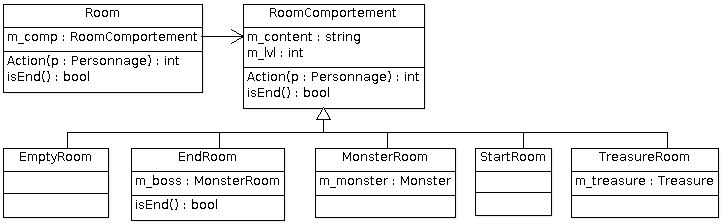
\includegraphics[width=15cm]{./Strategy_UML.png}
        \caption{\label{fig:Strategy_UML} UML : Pattern Strategy}
      \end{figure}

Le pattern strategy est utilisé pour gérer le comportement des salles (Figure \ref{fig:Strategy_UML}\footnotemark[1]).
Les salles peuvent changer de comportement au court du programme, ainsi au lieu de réécrire plusieurs fois la même choses (comme l'ouverture d'un coffre ou un combat) ceux-ci sont séparer dans différente classe pour une même méthode (action() dans notre cas).
Dans le déroulement normal du programme, une salle initialement comportant un monstre d'un certain niveau, si l'on rentre nous lançons le combat si nous gagnons alors la salle prend le comportement d'une salle de coffre.
Si nous ouvrons ce coffre alors par la même méthode action nous récupérons le trésor dedans et le comportement de la salle sera celle de la salle vide.

Ainsi, on évite une grosse classe lourde à gérer qui ferait la gestion du monstre potentiel avec celui d'un trésor avec la possibilité que ce soit celle de fin.
Et, nous évitons aussi un code dur à maintenir.
En utilisant ce pattern nous avons aussi une grande flexibilité, puisque, dans le comportement de la salle de fin, nous avons ajouté un comportement salle monstre pour ajouter un monstre sans réécrire la méthode de combat.
Mais ce comportement est géré en interne puisque la salle de fin n'est pas une salle de monstre comme les autres.
Celle-ci doit être repérée comme salle de fin et non juste une banale salle ayant un monstre.


    \subsection{Pattern State}
      \begin{figure}[h]
        \centering
        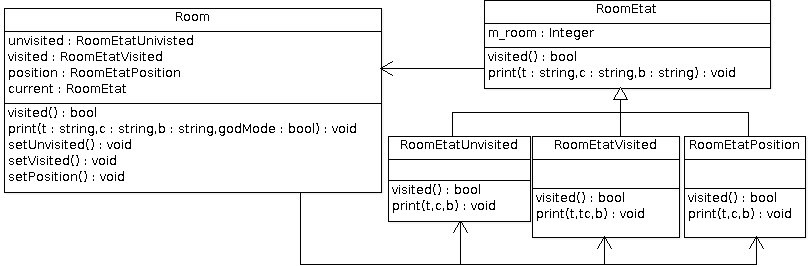
\includegraphics[width=15cm]{./State_UML.png}
        \caption{\label{fig:State_UML} UML : Pattern Abstract Factory}
      \end{figure}

Le pattern state est utilisé pour connaître l'état de la salle (Figure \ref{fig:State_UML}\footnotemark[1]).
Avec ce pattern on sait si c'est une salle qu'on a visité ou une salle qu'on ne connaît pas. Mais aussi si la salle est notre position actuelle.
Comme il peut y avoir beaucoup de changement d'état (si l'on repasse plusieurs fois sur une même case on change plusieurs fois l'état en EtatPosition en EtatVisite et inversement) on pré-charge les états à la création de l'instance puis on switch un simple pointeur pour changer d'état.

Le choix du pattern state est aussi pour une éventuelle amélioration, on pourrait ajouter un état fermé qui empêche de rentrer pour les X premiers tours.
Ou ajouter les certaines méthodes (comme Action) dans la partie l'état pour qu'elle soit exécutable seulement quand je suis dans l'état position.

    \subsection{Pattern Abstract Factory}
      \begin{figure}[h]
        \centering
        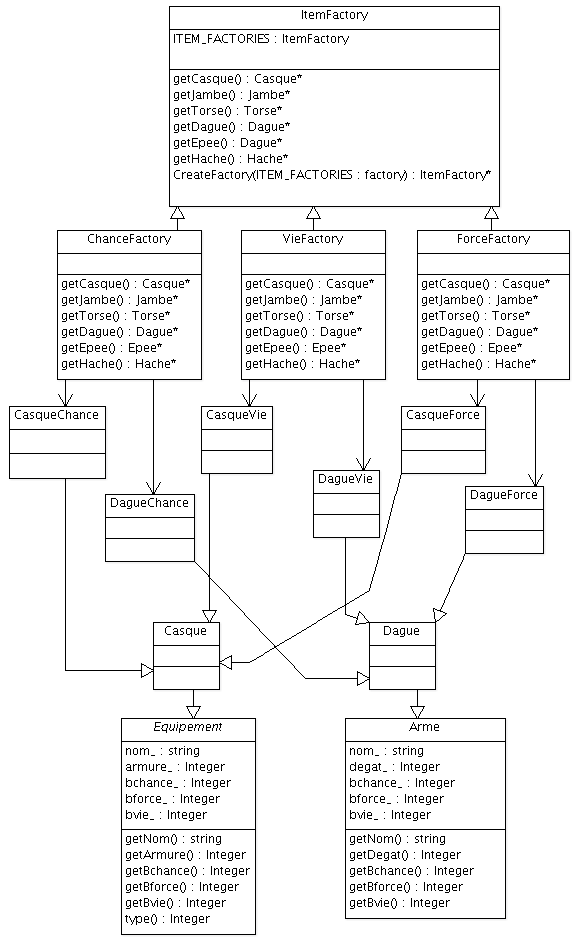
\includegraphics[width=11.5cm]{./Factory_UML.png}
        \caption{\label{fig:Factory_UML} UML : Pattern Abstract Factory}
      \end{figure}

Le pattern abstract factory utilisé ici permet la création des équipements et des armes pour le personnage.
Il est composé d'une classe abstraite ItemFactory, de 3 factory concrètes qui en découlent : ChanceFactory , ForceFactory et VieFactory
Ces factory permettent de créer différents types d'objets.6 classe abstraite d'objet : Dague, Epee, Hache, Casque, Jambe et Torse.
Ces 6 classes abstraites possèdent chacune 3 classes filles qui sont les objets concrets (Ex : EpeeVie , CasqueChance , JambeForce etc...).
Le fonctionnement de ce pattern est simple : La classe ItemFactory créer lors de l'appel de sa méthode une factory concrète en fonction du type passé en paramètre (CHANCEF, FORCEF, VIEF).
Ensuite cette factory concrète va créer des objets en fonction de la méthode appelée.
Par exemple une factory de type chance (ChanceFactory) créera un item de type HacheChance si la méthode getHache() est appelée.

L'utilisation de ce pattern pour gérer les équipements et armes permet une bonne encapsulation des classes lors de leur création.
Cela facilite aussi grandement la création des équipements et des armes en les faisant créer par la factory.
Dans la mesure ou nous voudrions rajouter des nouvelles armes ou équipements ou même un nouveau type de bonus(Agilité par exemple) le code existant n'aurait pas besoin de beaucoup de modification.
Le pattern Abstract Factory est donc en parfaite adéquation avec la gestion des équipements pour ce type de jeu et donc pour notre programme.

Sur le diagramme UML (Figure \ref{fig:Factory_UML}), nous n'avons pas mis toutes les classes abstraites et concrètes des Armes et Équipements car cela prenait beaucoup de place.
Il y a donc Jambe, JambeChance , JambeForce, JambeVie, Torse, TorseChance, TorseForce, TorseVie, Epee, EpeeChance, EpeeForce, EpeeVie, Hache, HacheChance, HacheForce et HacheVie qui manque sur la diagramme, en effet , elles sont très proche de Dague, Casque et leurs classes filles déjà présentes.


  \subsection{Pattern Decorator}
    \begin{figure}[h]
      \centering
      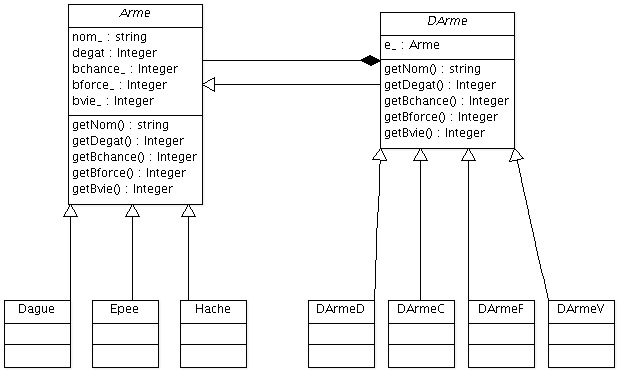
\includegraphics[width=15cm]{./Decorator_UML.png}
      \caption{\label{fig:Decorator_UML} UML : Pattern Decorator}
    \end{figure}

Ce programme implémente deux Decorators différent. Un pour les Armes et un pour les Équipements. Ici le diagramme UML est celui du decorator d'arme néanmoins celui des équipements est quasiment identique à celui-ci.

Le pattern decorator utilisé ici permet de décorer les objets précédemment créé par les factory.
Ainsi un objet "Casque de Vie" donnant +X à la vie du personnage pourra être décoré en "Casque de Vie+1" donnant +X+Y à la vie du personnage, ou bien en "Casque de Vie de Force" donnant +X à la vie et +Y à la force du personnage.
Tout cela selon les décorations appliquées à l'objet.
Ce pattern est composé d'une classe DArme qui hérite de la classe abstraite Arme et qui possède un attribut Arme.
Grâce à celui-ci des bonus sont ajoutés à l'objet lors de sa décoration et son nom change.
Pour le nom, on ajoute respectivement "de Force", "de Vie", "de Chance", "de Dégât" ou "Puissante" si l'on décore avec de la force, de la vie, de la chance, du dégât ou de l'armure.
Ensuite si le nom de l'objet est déjà composé d'une de ces chaînes et que l'on le décore à nouveau l'objet qui devrait devenir par exemple :
"Epee de Force de Force", il deviendra "Epee de Force+1 " puis "Epee de Force+2" selon le nombre de fois où il est décoré.
Ses bonus seront aussi modifiés.
Le décorator d'Equipement fonctionne exactement de la même manière que celui d'Arme mais avec un bonus d'armure plutôt que de dégâts.

L'utilisation de ce pattern nous permet de créer un très grand nombre d'objet différent sans avoir à créer des centaines de classes. Ainsi pas besoin d'avoir une classe spécifique pour créer un objet du genre "Epee Puissante+2 de Force+9 de Vie+2 de Chance+4"
En effet, il suffit de redécorer l'objet que l'on souhaite pour augmenter ses bonus.
Comme pour le pattern Abstract Factory, il sera très simple avec ce pattern de rajouter des types d'équipements et des types de bonus sans avoir à trop modifier le code existant. C'est donc un pattern qui colle parfaitement avec ce que nous voulions faire.
De plus la combinaison de ces deux pattern (Abstract Factory et Decorator) créer une très bonne synergie pour la création de nombreux objets.

  \newpage
  \section{Conclusion}
Pour finir même si l'implémentation du jeu c'est plutôt bien déroulé, quelques problèmes nous ont quelques fois ralentis.
Par exemple, au niveau du pattern Decorator où lorsqu'un objet était décoré 10 fois ou plus, il devenait très long de recréer le nom de cet objet.
Ce problème venait du fait que la méthode qui reconstruit le nom des objets s'appelait récursivement et amenait à des temps d'exécution extrêmement long.
Pour régler ce problème nous avons dû calculer le nom de l'objet à la création de l'objet plutôt que de recalculer lors de l'appel de la méthode getNom de l'objet.

Pour la suite du programme et pour l'améliorer, il y a plusieurs choses que nous pourrions faire.
Tout d'abord, l'implémentation d'une interface graphique pour le labyrinthe et de sprite pour le joueur et les monstres pourraient rendre le jeu beaucoup plus immersif que l'aspect simpliste de la console.
Ensuite la création d'un inventaire pour le personnage serait envisageable et permettrait l'apparition de consommable tel des potions qui pourrait renforcer le personnage pour un certain temps ou nombre de combats.
Les combats pourraient être aussi améliorés afin d'impliquer le joueur qui, ici, doit juste attendre de voir s’il gagne ou s’il perd.
Enfin, plusieurs niveaux de labyrinthe et des monstres de plus en plus fort permettrait d'améliorer grandement la durée d'une partie.

En conclusion, ce projet nous aura permis de voir l'utilité des Design Pattern dans un contexte "réel" et de remarquer que si ils sont bien utilisés ils permettent de gagner énormément de temps. De plus le code est largement simplifié par leur utilisation et un problème que l'on aurait pu résoudre avec de très nombreuses classes se résous finalement en très peu de place.
De plus, le fait que le projet soit libre, pas de consigne imposée (mis à part l’inclusion des 4 patterns), nous a permis de nous investir plus facilement dans l'implémentation du programme.
En effet, un sujet imposé et beaucoup moins motivant, celui-ci ne laissant que très peu de place à l'imagination.
Par contre, il est beaucoup plus difficile de commencer un projet lorsqu'il est libre. Car n'ayant pas de fil directeur il est parfois un peu dur de savoir ce qu'il faut commencer à implémenter et ce qui peut attendre. Surtout lorsque l’on n’a pas encore une idée fixe sur le programme.
\newpage
\begin{figure}[h]
        \centering
        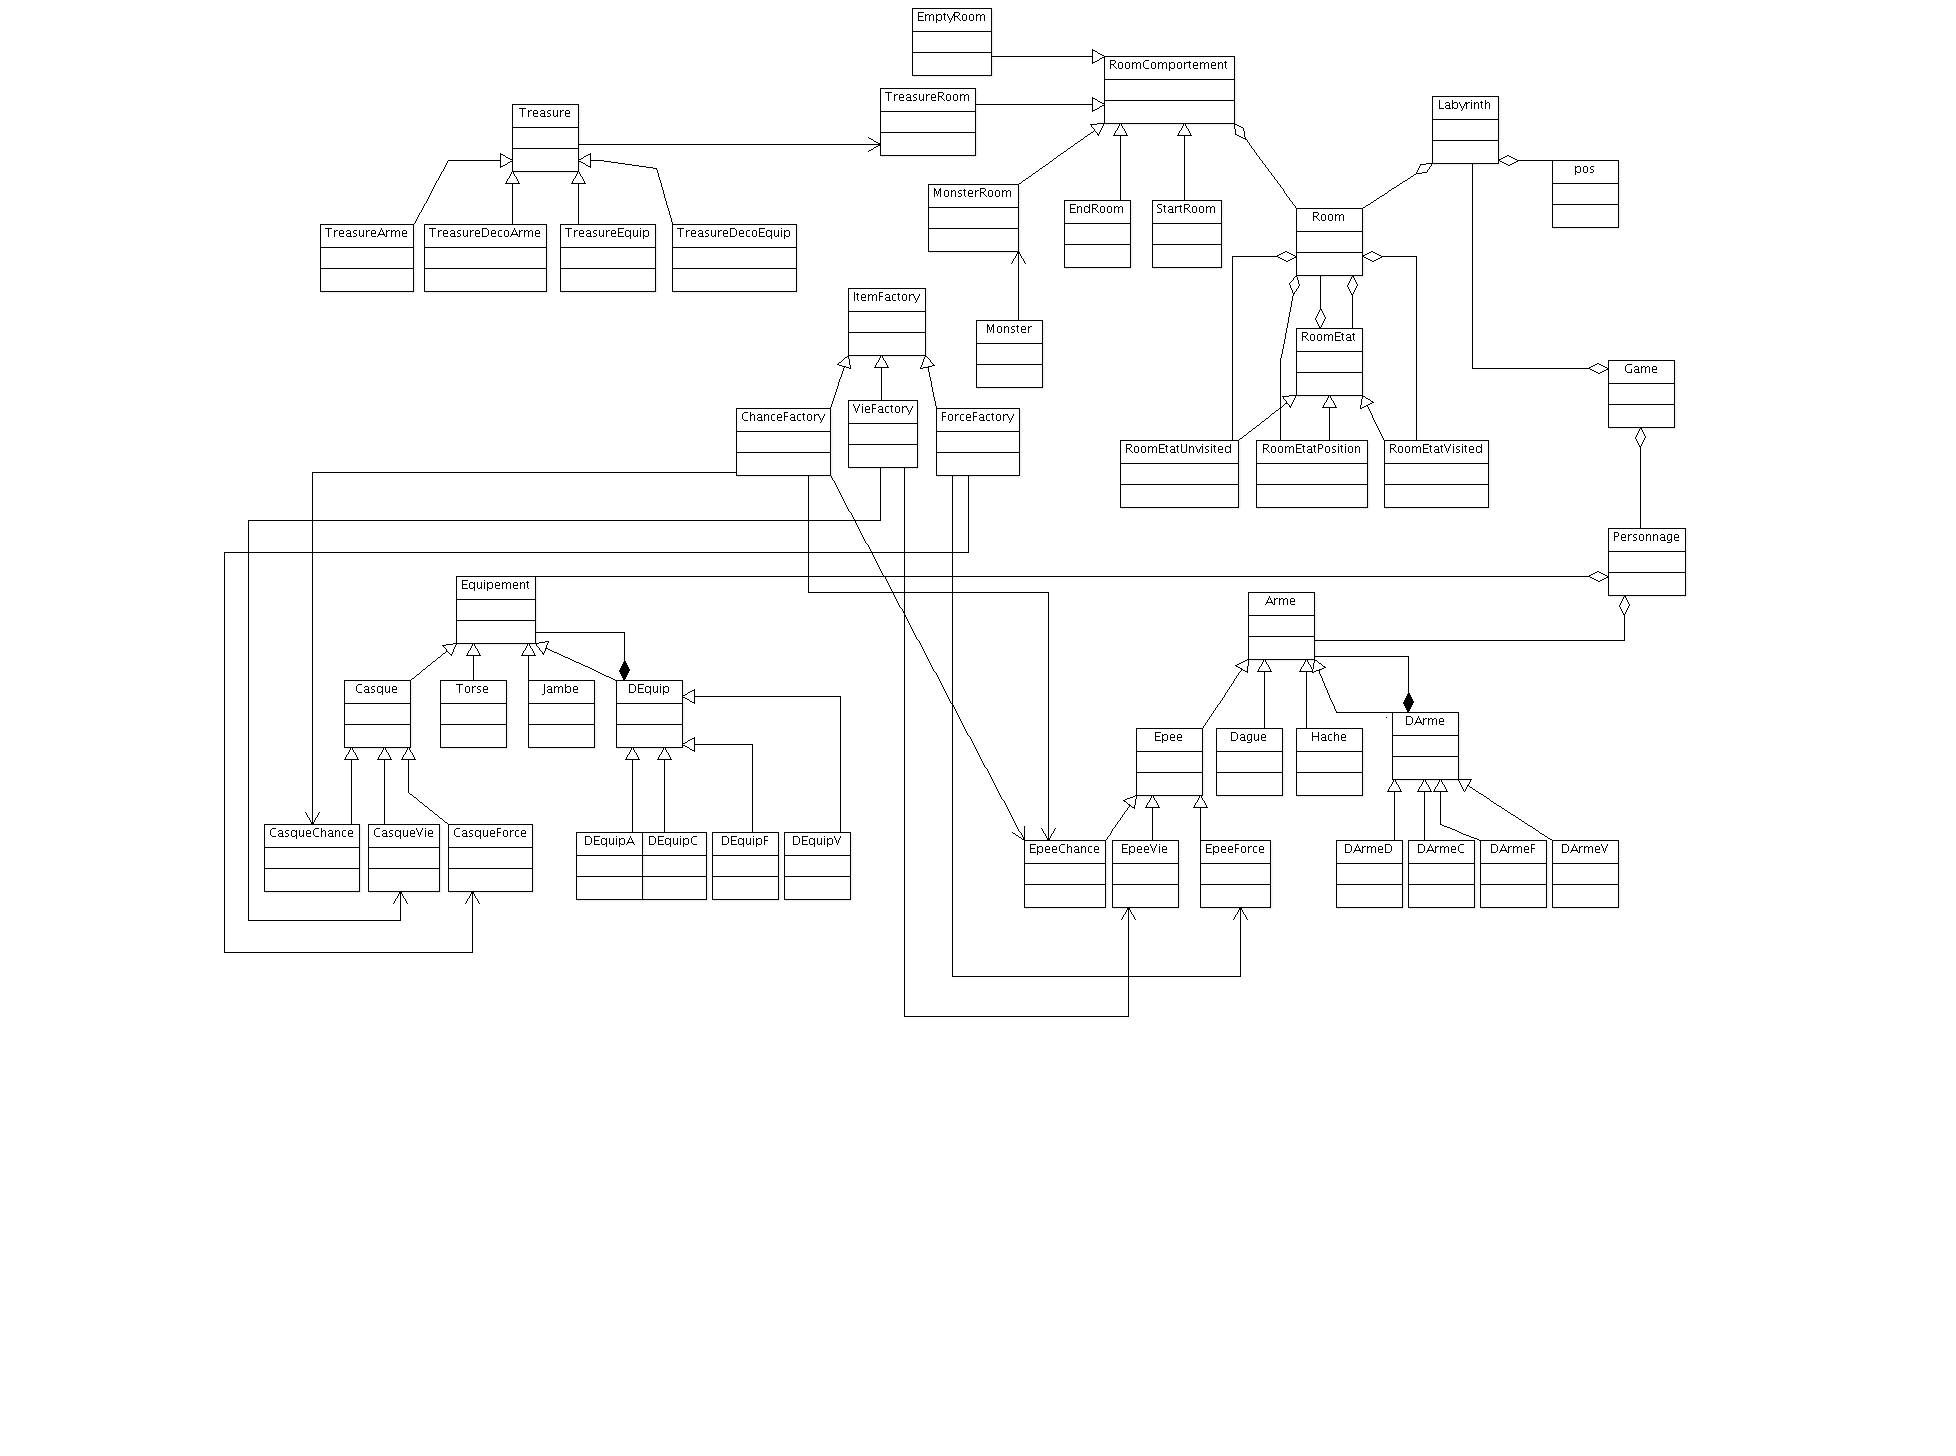
\includegraphics[angle=90,width=17cm]{./DiagrammeDeClasse.png}
        \caption{\label{fig:diagClasse}Diagramme de classe}
      \end{figure}

\end{document}

